\documentclass[a4paper, 11pt]{article}
\usepackage{float}
\usepackage{subfig}
\usepackage{graphicx} % Required to insert images
\usepackage{hyperref}
\title{
\begin{Huge}\textbf{Using Intel Advisor on Sunbird} \end{Huge} \\

\includegraphics[width = 65mm]{logos/sa2c.pdf}\\[8ex]
\begin{large} \textbf{Swansea Academy of Advanced computing} \end{large} \\
\normalfont \normalsize
\begin{normalsize} Swansea University \end{normalsize} \\
}
\author{Dr. Benjamin Thorpe, RSE Swansea University} % Your name
\date{\today} % Today's date or a custom date
\begin{document}
\begin{titlepage}
\maketitle
\vfill
\end{titlepage}
\section{Introduction}
Intel Advisor is a useful tools for examining the performance of C, C++ and Fortran code and can provide useful information and insight on how to improve your code to get the most out of the available hardware. 

If you are examining code running on your personal machine you would normally use the GUI provided by Intel as part of its parallel studio software suite. However, whilst you can in principle run graphical software on Sunbird (via X11 forwarding or on VNC login nodes) it is not recommended in this case since the profiler and code need to be run on the compute nodes which is not possible within a VNC setup.

Therefore, in this short guide we will explain how to Intel Advisor correctly on Sunbird with SLURM using the command line interface (CLI). We will then explain how to export the final data either in Intel's proprietary format, for analysis on your personal machine (via parallel studio) or in text plain format (e.g. a csv file) for processing/analysis in your software of choice.
        
\section{Setup}
To use Intel Advisor on Sunbird we simply need to load the modules for the Intel compiler and Intel parallel studio and then source the advixe-vars script.
\begin{verbatim}
module load compiler/intel/2019/5
module load intel-psx/2019.5
source /apps/compilers/intel/2019.5/advisor/advixe-vars.sh
\end{verbatim}
\section{Running Basic Analysis}
To perform our analysis we will be using the \verb+advixe-cl+ command this command allows us to perform all the different types of analysis that are available via the GUI and as such has a large number of options.

Here we will discuss the some useful useful options to get started (to browse through all of the available opinions use \verb+advixe-cl --help+). 

To perform a basic hotpot analysis we use the collect option with the argument survey as follows:
\begin{verbatim}
 advixe-cl --collect=survey -- ./myApplication -options
 \end{verbatim}
 
 By default advisor creates a directory advi in the current working directory to store the advisor project, containing the analysis results we can specify a different directory if needed with the optional argument \verb+--project-dir+. 
 
 It also assumes the binary containing debug symbols and the source code are in the current working directory. If this is not the case we can use the optional argument \verb+--search-dir+, to specify directories containing the source code and compiled binaries.
 
However, \verb+--search-dir+ has its own sub options to specify what to look for. These are \verb+ all:, src:, bin: and sym:+ alongside \verb+r+ to search recursively. For example:

\begin{verbatim}
 advixe-cl --collect=survey --project-dir=./advisor \
  --search-dir src:r=./src --search-dir bin:=./rundir \
   -- rundir/myApplication -options
\end{verbatim}
 
This tells advisor to put the project in the directory \verb+advisor+ and search for source files recursively starting at \verb+src+ and to search for the binary containing the debug symbols in \verb+rundir+.

We can also ask advisor to track the number of loop iterations and calls to functions (tripcounts) with:
\begin{verbatim}
 advixe-cl --collect=tripcounts -- ./myApplication -options
 \end{verbatim}

alongside same sub-options as we did with survey to control output and search destinations.

Once we have run the analysis we have two options for analysing the data.

\begin{enumerate}
\item Copy the project directory, sources and binary to another machine and open the project in Intel advisor.
\item Use the report option to output the data to a text file for analysis as we see fit 
\end{enumerate}
 
 For option 2 the syntax is as follows:
 \begin{verbatim}
advixe-cl --report=survey --format=csv --project-dir=./advisor \
--report-output ./report.csv
\end{verbatim}

This outputs the results into a csv file specified by \verb+--report-output+, if this is omitted it will be sent to standard output. By default it uses commas for the delimiter this can be changed with \verb+--csv-delimiter+. It also only shows loops by default you can show functions using \verb+-show-functions+.

Some other useful options include \verb+-filter=<column_name>+ to output only specific columns and \verb+-s=<column_name>+ to sort results in ascending order by the named column (or \verb+-S+ to sort in descending order).

We can also add the tripcounts data to the report using 
 \begin{verbatim}
advixe-cl --report=tripcounts --format=csv --report-output ./report.csv
\end{verbatim}

\paragraph{Notes about using MPI} When using the \verb+--collect+ with non-intel mpi we need to use the aditional option \verb+--trace-mpi+. From here both Intel and non-Intel mpi can be called as:
 \begin{verbatim}
<mpilauncher> [options] advixe-cl [options] \
-- <application> [arguments] 
\end{verbatim}

You do not need to specify an output directory since this will create a directory for each rank called rank.n. you can then view the data using the GUI as before. You can also extract results using \verb+--report+. By default you get data for all the ranks. However, you can get results for a specific rank using the option \verb+--mpi-rank=n+. 

Intel mpi also has the option \verb+-gtool+ this allows you to profile on only select ranks, amongst other things. Details for it's usage can be found here: 

\url{https://software.intel.com/content/www/us/en/develop/articles/using-intel-advisor-and-vtune-amplifier-with-mpi.html}

\section{Roofline Analysis}
To perform a roofline analysis one simply needs to run a survey followed by tripcounts analysis. However, we need to add a new option \verb+--flop+ to the tripcounts collection to tell advisor to collect information on flops for each loop and function.
 \begin{verbatim}
 advixe-cl --collect=survey -- ./myApplication -options
advixe-cl --collect=tripcounts --flop -- ./myApplication -options
\end{verbatim}

Alternatively in advisor 2019 a roofline option was added to collect as a shortcut
 \begin{verbatim}
 advixe-cl --collect=roofline -- ./myApplication -options
\end{verbatim}

To analyse the data we have 3 choices
\begin{itemize}
\item open the advisor project using the GUI on a different machine
\item generate an HTML interactive roofline plot \verb+--report=roofline+
\item output the raw data for plotting using \verb+--report=tripcounts+.
\end{itemize}

For option two we have several flags we can use to control what data is plotted. The standard usage is as follows:
\begin{verbatim}
advixe-cl --report=roofline --project-dir=./advisor \
--report-output ./roofine.html
\end{verbatim}

The default behaviour is to plot the data for only floating point operations with all the memory roofs. If we only want integer operations or combined data we can use \verb+----data-type+ followed by either int or mixed. To specify which memory levels to plot we can use \verb+--memory-level+ followed by a list of levels to include (separated by underscores) for example \verb+--memory-level=DRAM_L1+ will just plot DRAM and L1 cache or \verb+--memory-level=L2_L3+ will just plot L2 and L3 cache.
 

For option three, we need to obtain the arithmetic intensity and flops data. to do this we can use the option \verb+--show-all-data+. This tells advisor to output all the raw data it has collected. Most of this information is not relevant so its recommended you either write a script  to parse the necessary data or use the \verb+--filter+ option. The repo where this document came from contains an example python script "roofline.py" that shows an example of this using pandas.

The columns we are interested in are (apologies if these names are confusing blame Intel):
\begin{itemize}
\item Self GFLOPS (floating point operations per second)
\item Self GFLOP (total number of floating point operations) 
\item Self AI (calculated arithmetic intensity for floating point operations) 
\item Self Memory GB (total memory accessed in GB)
\item Self GB/s (total memory accessed per second)
\end{itemize}

Advisor 2019 and above also track integer operations (INTOPs) and thus include the following additional columns.

\begin{itemize}
\item Self GINTOPS (integer operations per second)
\item Self Giga OPS (combined total integer and floating point operations per second)
\item  Self GINTOP (total number of integer operations)
\item Self Giga OP (combined total integer and floating point operations)
\item Self INT AI (calculated arithmetic intensity for integer operations)
\item Self Overall AI (calculated combined arithmetic intensity)
\end{itemize}

To generate a roofline plot we can then simply plot Self GFLOPS against Self AI with a log-log scale. This information on its own however is not very useful. The final step is to extract the hardware roofs. This is achieved using:
 \begin{verbatim}
advixe-cl --report=roofs --format=csv --report-output ./roofs.csv
\end{verbatim}
This gives numbers for each of the various hardware limits (L1 cache, L2 cache, DRAM etc). These are labelled in the type column as either memory or compute. The compute values define horizontal lines at $y=compute$ for the various cpu bottlenecks. The memory values (generally L1, L2 and L3 cache, and DRAM) define the slope of a line from starting at the origin and stopping at is intersection with the highest compute line (see figure \ref{roofline}). 

These do However need separating into three groups: multithreaded, vector and scalar. These are labelled in the roofs.csv file and again you may want some script to automate this for you. The example python script "roofline.py" shows one possible way of achieving this using pandas although there are doubtless many alternatives.

\begin{figure}
    \centering
    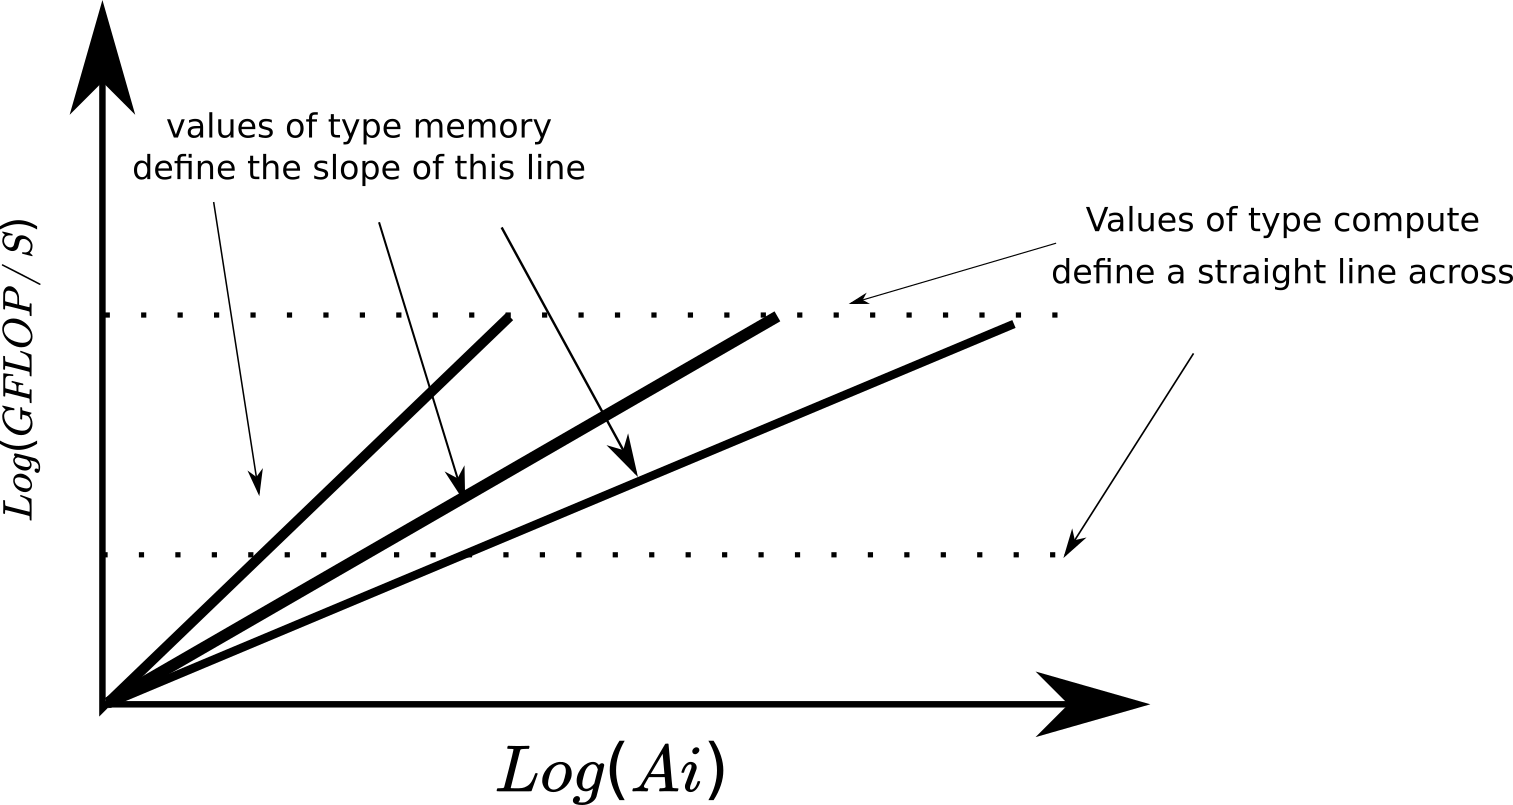
\includegraphics[width=0.5\textwidth]{roofline.png}
    \caption{\label{roofline}}
\end{figure}

\end{document}


